\documentclass[12pt,a4paper,english]{article}

\usepackage[a4paper,hmargin=25mm,vmargin=25mm]{geometry}
\usepackage[utf8]{inputenc}
\usepackage[backend=biber,style=numeric,sortcites,firstinits=true]{biblatex}
\usepackage[skip=5pt, indent=15pt]{parskip}
\usepackage[hidelinks]{hyperref}
\usepackage{babel}
\usepackage[T1]{fontenc}
\usepackage{indentfirst}
\usepackage{textcomp}
\usepackage{url}
\usepackage{csquotes}
\usepackage{graphicx}
\usepackage{float}
\usepackage{amsmath}
\usepackage{amssymb}
\usepackage{amsfonts}

\urlstyle{sf}
\addbibresource{./refs.bib}
\graphicspath{ {./figures/} }

\title{\textbf{OCES5303} \linebreak Assignment 1}
\author{Jonas Mathisrud Sterud}

\begin{document}
    \maketitle

    \begin{abstract}
        Argo is an international program collecting data from the ocean at various depths using robotic instruments drifting with ocean currents.
        \cite{argo}

        In this assignemnt, we will explore the dataset, and perform linear regression to see if \dots.
    \end{abstract}

    \begin{figure}[H]
        \begin{center}
            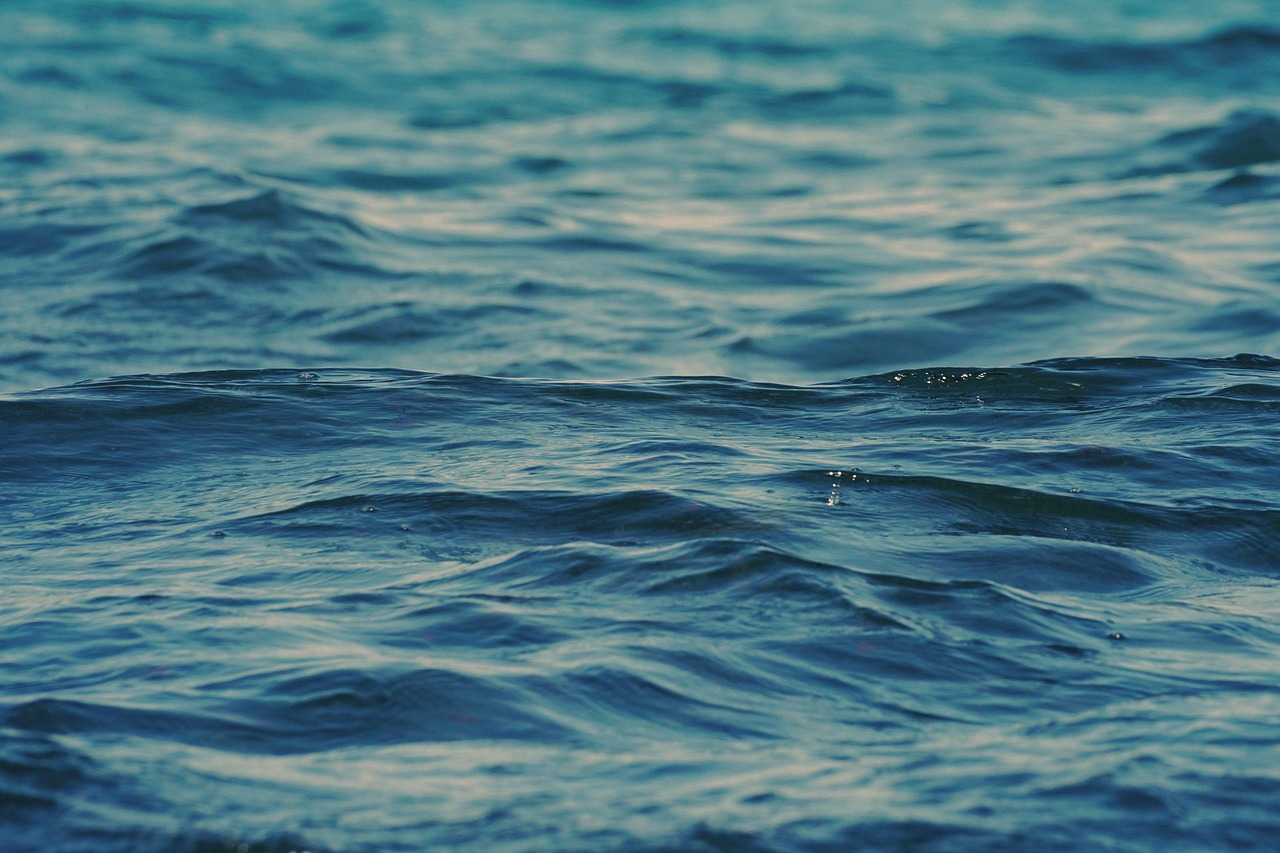
\includegraphics[width=13cm]{cover.jpg}
        \end{center}
    \end{figure}

    \newpage
    \tableofcontents
    \newpage

    \section{Introduction}

    \dots

    \section{Acknowledgments}

    \begin{itemize}
        \item[] ``These data were collected and made freely available by the International Argo Program and the national programs that contribute to it.  (https://argo.ucsd.edu,  https://www.ocean-ops.org).  The Argo Program is part of the Global Ocean Observing System.''
    \end{itemize}
    
    

    \noindent Argo (2000). Argo float data and metadata from Global Data Assembly Centre (Argo GDAC). SEANOE. https://doi.org/10.17882/42182

    \newpage
    \printbibliography
\end{document}
